\section{极限}

本节阐述微积分的基础概念——极限。
充分理解极限的概念,学会用极限的概念证明函数极限的存在性。

本节要点:
\begin{itemize}
    \item 掌握极限的概念;
    \item 深入理解夹逼定理;
    \item 推导两个重要的极限:$\underset{x\rightarrow 0}{\lim}\frac{\sin x}{x}=1$、$\underset{x\rightarrow \infty}{\lim}\left( 1+\frac{1}{x} \right) ^x=e$。
\end{itemize}

%============================================================
\subsection{极限的概念}

\begin{definition}[极限]
设$f\left( x \right) $在某去心邻域$N\left( \hat{x}_0 \right) $内有定义,对于$\forall \varepsilon >0$,总存在$\delta >0$,使得当$x\in N\left( \hat{x}_0,\delta \right) $时$\left| f\left( x \right) -A \right|<\varepsilon $,则称$A$为{\bf 当$x\rightarrow x_0$时$f\left( x \right) $的极限(limit)},记作$\underset{x\rightarrow x_0}{\lim}f\left( x \right) $,即:
\[
\underset{x\rightarrow x_0}{\lim}f\left( x \right) :=A
\]
\end{definition}

简单来讲,即$0<\left| x-x_0 \right|<\delta \Rightarrow \left| f\left( x \right) -A \right|<\varepsilon $。
式中的$x_0$和$A$是事先给定,$\varepsilon $和$\delta $是要确定相互关系。
判断$f\left( x \right) $在$x_0$是否有极限就是通过将$\left| f\left( x \right) -A \right|<\varepsilon $转化成$0<\left| x-x_0 \right|<\delta $,找出$\varepsilon $和$\delta $的关系,如果能找到彼此的关系,就证明了该极限的存在。

\begin{tcolorbox}
一元函数的极限和多元函数一样,都有“方向”这个概念。
一元函数中的方向比较简单,只有左右两个方向。
\end{tcolorbox}

\begin{definition}[左极限]
设$f\left( x \right) $在某去心邻域$N\left( \hat{x}_0 \right) $内有定义,对于$\forall \varepsilon >0$,总存在$\delta >0$,使得当$x\in \left( x_0-\delta ,x_0 \right) $时$\left| f\left( x \right) -A \right|<\varepsilon $,则称$A$为{\bf 当$x\rightarrow x_0$时$f\left( x \right) $的左极限},记作$\underset{x\rightarrow {x_0}^-}{\lim}f\left( x \right) $,即:
\[
\underset{x\rightarrow {x_0}^-}{\lim}f\left( x \right) :=A
\]
\end{definition}

\begin{definition}[右极限]
设$f\left( x \right) $在某去心邻域$N\left( \hat{x}_0 \right) $内有定义,对于$\forall \varepsilon >0$,总存在$\delta >0$,使得当$x\in \left( x_0,x_0+\delta \right) $时$\left| f\left( x \right) -A \right|<\varepsilon $,则称$A$为{\bf 当$x\rightarrow x_0$时$f\left( x \right) $的右极限},记作$\underset{x\rightarrow {x_0}^+}{\lim}f\left( x \right) $,即:
\[
\underset{x\rightarrow {x_0}^+}{\lim}f\left( x \right) :=A
\]
\end{definition}

极限的定义告诉我们,如果函数的极限存在,说明我们总能找到一个去心邻域$N\left( \hat{x}_0 \right) $,使得该邻域内的 “更加接近”常数$A$。
数学上,极限描述一个“界”。
极限的物理意义在于考察一个物理量能不能达到一个稳定的状态,以及该稳定状态下值是多少。
极限概念在给解决这类物理问题时提供了数学基础。

\begin{theorem}[柯西判别准则]
当$x\rightarrow x_0$时函数$f\left( x \right) $有极限的充要条件是:对于$\forall \varepsilon >0$,总存在$\delta >0$,使得当$x_1,x_2\in N\left( \hat{x}_0,\delta \right) $时,恒有:
\[
\left| f\left( x_1 \right) -f\left( x_2 \right) \right|<\varepsilon
\]
\end{theorem}

柯西判别准则的优势在于可以不知道具体的极限值而对函数是否有极限进行判断。
同时,也可以作为极限的定义。

%============================================================
\subsection{极限的运算法则}

\begin{align*}
\begin{matrix}
	\underset{x\rightarrow x_0}{\lim}k=k \hfill & \underset{x\rightarrow x_0}{\lim}\left[ f\left( x \right) +g\left( x \right) \right] =\underset{x\rightarrow x_0}{\lim}f\left( x \right) +\underset{x\rightarrow x_0}{\lim}g\left( x \right) \hfill \\
	\underset{x\rightarrow x_0}{\lim}x=x_0 \hfill & \underset{x\rightarrow x_0}{\lim}\left[ f\left( x \right) -g\left( x \right) \right] =\underset{x\rightarrow x_0}{\lim}f\left( x \right) -\underset{x\rightarrow x_0}{\lim}g\left( x \right) \hfill \\
	\underset{x\rightarrow x_0}{\lim}kf\left( x \right) =k\underset{x\rightarrow x_0}{\lim}f\left( x \right) \hfill & \underset{x\rightarrow x_0}{\lim}\left[ f\left( x \right) \cdot g\left( x \right) \right] =\underset{x\rightarrow x_0}{\lim}f\left( x \right) \cdot \underset{x\rightarrow x_0}{\lim}g\left( x \right) \hfill \\
	\underset{x\rightarrow x_0}{\lim}\left[ f\left( x \right) \right] ^n=\left[ \underset{x\rightarrow x_0}{\lim}f\left( x \right) \right] ^n \hfill & \underset{x\rightarrow x_0}{\lim}\frac{f\left( x \right)}{g\left( x \right)}=\frac{\underset{x\rightarrow x_0}{\lim}f\left( x \right)}{\underset{x\rightarrow x_0}{\lim}g\left( x \right)} \hfill \\
\end{matrix}
\end{align*}

这些运算法则告诉我们,极限是一个线性运算。
同时说明,多项式在某点的极限等于多项式在该点的函数值。

%============================================================
\subsection{极限的定理}

极限的定理都是围绕着极限的定义展开。
描述存在极限的函数的性质,有界、保号、夹逼、单调。

\begin{theorem}[左右极限定理]
\[
\underset{x\rightarrow x_0}{\lim}f\left( x \right) =A\Leftrightarrow \underset{x\rightarrow {x_0}^-}{\lim}f\left( x \right) =\underset{x\rightarrow {x_0}^+}{\lim}f\left( x \right) =A
\]
\end{theorem}

\begin{theorem}[唯一性定理]
若$\underset{x\rightarrow x_0}{\lim}f\left( x \right) =A$,则$A$唯一。
\end{theorem}

\begin{theorem}[有界性定理]
若$\underset{x\rightarrow x_0}{\lim}f\left( x \right) =A$,则有$\forall M>0,\exists \delta >0$,使得$\forall x\in N\left( \hat{x}_0,\delta \right) \Rightarrow \left| f\left( x \right) \right|\leqslant M$成立,即收敛函数必有界。
\end{theorem}

\begin{tcolorbox}
注意,有界不一定收敛,如$\sin x$。
\end{tcolorbox}

\begin{theorem}[单调有界定理]
单调有界函数必存在极限。
\end{theorem}

\begin{theorem}[局部保号性定理]
若$\underset{x\rightarrow x_0}{\lim}f\left( x \right) =A>0$(或$<0$),则必有$\exists \delta >0$,使得$\forall x\in N\left( \hat{x}_0,\delta \right) \Rightarrow f\left( x \right) >0$(或$<0$)成立。
\end{theorem}

\begin{corollary}
\[
f\left( x \right) \geqslant 0,\underset{x\rightarrow x_0}{\lim}f\left( x \right) =A\Rightarrow A\geqslant 0
\]
\end{corollary}

\begin{corollary}
\[
f\left( x \right) \geqslant g\left( x \right) ,\underset{x\rightarrow x_0}{\lim}f\left( x \right) =A,\underset{x\rightarrow x_0}{\lim}g\left( x \right) =B\Rightarrow A\geqslant B
\]
\end{corollary}

\begin{theorem}[夹逼定理]
若在去心邻域$N\left( \hat{x}_0,\delta \right) $内,有$g\left( x \right) \leqslant f\left( x \right) \leqslant h\left( x \right) $,$\underset{x\rightarrow x_0}{\lim}g\left( x \right) =\underset{x\rightarrow x_0}{\lim}h\left( x \right) =A$,则$\underset{x\rightarrow x_0}{\lim}f\left( x \right) =A$。
\end{theorem}

\begin{proof}
对于$\forall \varepsilon >0$,必存在邻域$N\left( \hat{x}_0,\delta _g \right) $,有$x\in N\left( \hat{x}_0,\delta _g \right) \Rightarrow \left| g\left( x \right) -A \right|<\varepsilon $,也必存在邻域$N\left( \hat{x}_0,\delta _h \right) $,有$x\in N\left( \hat{x}_0,\delta _h \right) \Rightarrow \left| h\left( x \right) -A \right|<\varepsilon $。
所以,令$\delta _f=\min \left\{ \delta ,\delta _g,\delta _h \right\} $,当$N\left( \hat{x}_0,\delta _f \right) $时,根据$g\left( x \right) \leqslant f\left( x \right) \leqslant h\left( x \right) $必有:
\[
A-\varepsilon <g\left( x \right) \leqslant f\left( x \right) \leqslant h\left( x \right) <A+\varepsilon
\]
\end{proof}

上述定理中,唯有夹逼定理是定量性的定理。
该定理用于计算极限,在多元函数中的应用也十分广泛。

%============================================================
\subsection{两个重要的极限}

{\bf 计算$\underset{x\rightarrow 0}{\lim}\frac{\sin x}{x}$}

总体思路,用夹逼定理计算。

\begin{figure}[h]
\centering
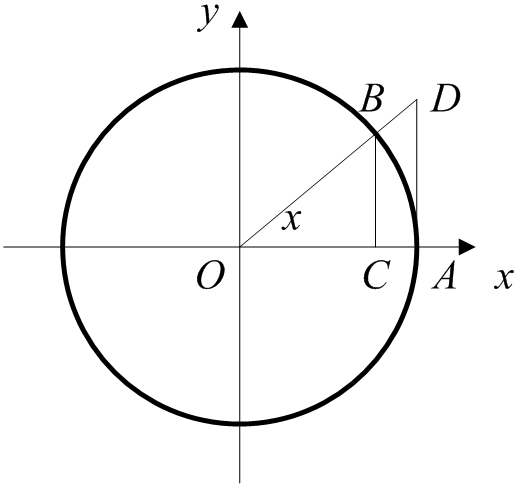
\includegraphics[height=3.5cm]{1.1.png}
\end{figure}

考虑单位圆,{\it OD}和{\it x}轴夹角 。
考察三角形{\it OBC}、扇形{\it OAB}、三角形{\it OAD},三者面积有关系:
\begin{align*}
&\because S_{OBC}<S_{OAB}<S_{OAD} \\
&\therefore \frac{1}{2}\sin x\cos x<\pi \cdot \frac{x}{2\pi}<\frac{1}{2}\tan x \\
&\therefore \cos x<\frac{\sin x}{x}<\frac{1}{\cos x}
\end{align*}
对于余弦函数有$\underset{x\rightarrow 0}{\lim}\cos x=1$,由夹逼定理得:
\[
\underset{x\rightarrow 0}{\lim}\frac{\sin x}{x}=1
\]

注意,这里不能用线段{\it BC}长度、弧{\it AB}长度、线段{\it AD}长度的关系$BC<\overset\frown{AB}<AD$。
因为$\overset\frown{AB}<AD$不是那么显而易见,需要证明。

\begin{tcolorbox}
该极限将三角函数和多项式函数联系起来。
其值是一个计算得到的数值。
\end{tcolorbox}

{\bf 计算$\underset{x\rightarrow \infty}{\lim}\left( 1+\frac{1}{x} \right) ^x$}

还是用夹逼定理。
构造一个数列$x_n=\left( 1+\frac{1}{n} \right) ^n$。
用有界定理推导极限$\underset{n\rightarrow \infty}{\lim}\left\{ x_n \right\} $存在,证明略,并记为$e$。
\begin{align*}
&\because x>0\Rightarrow n\leqslant x\leqslant n+1 \\
&\therefore \left( 1+\frac{1}{1+n} \right) ^n<\left( 1+\frac{1}{x} \right) ^n\leqslant \left( 1+\frac{1}{x} \right) ^x\leqslant \left( 1+\frac{1}{n} \right) ^x<\left( 1+\frac{1}{n} \right) ^{n+1} \\
&\because \begin{cases}
	\underset{n\rightarrow \infty}{\lim}\left( 1+\frac{1}{1+n} \right) ^n=\underset{n\rightarrow \infty}{\lim}\frac{\left( 1+\frac{1}{1+n} \right) ^{n+1}}{1+\frac{1}{1+n}}=e\\
	\underset{n\rightarrow \infty}{\lim}\left( 1+\frac{1}{n} \right) ^{1+n}=\underset{n\rightarrow \infty}{\lim}\left[ \left( 1+\frac{1}{1+n} \right) ^n\left( 1+\frac{1}{1+n} \right) \right] =e\\
\end{cases} \\
&\therefore \underset{x\rightarrow +\infty}{\lim}\left( 1+\frac{1}{x} \right) ^x=e
\end{align*}
同理可证明$\underset{x\rightarrow -\infty}{\lim}\left( 1+\frac{1}{x} \right) ^x=e$。
由左右极限存在且相等得该极限存在且:
\[
\underset{x\rightarrow \infty}{\lim}\left( 1+\frac{1}{x} \right) ^x
\]

\begin{tcolorbox}
注意,该极限的值$e$是一个定义值。
该极限把指数函数和幂函数联系起来。
对于幂指函数的极限,基本都会有$e$的影子。
\end{tcolorbox}




